\documentclass[11pt,a4paper]{article}
\usepackage[margin=2.3cm]{geometry}
\usepackage{amsmath,amssymb,amsthm,mathtools}
\usepackage{algorithm,algpseudocode}
\usepackage{booktabs,graphicx,enumitem,xcolor}
\usepackage[colorlinks=true,linkcolor=blue!50!black,citecolor=green!40!black,urlcolor=blue!50!black]{hyperref}

\newtheorem{theorem}{Theorem}
\newtheorem{lemma}{Lemma}
\newtheorem{corollary}{Corollary}
\newtheorem{proposition}{Proposition}
\theoremstyle{definition}
\newtheorem{definition}{Definition}
\newtheorem{problem}{Problem}
\theoremstyle{remark}
\newtheorem{remark}{Remark}

\newcommand{\N}{\mathbb{N}}
\newcommand{\Z}{\mathbb{Z}}
\newcommand{\E}{\mathbb{E}}
\newcommand{\Prob}{\Pr}
\newcommand{\eps}{\varepsilon}
\newcommand{\ind}{\mathbf{1}}
\newcommand{\rt}{\tilde r}
\DeclarePairedDelimiter{\floor}{\lfloor}{\rfloor}
\DeclarePairedDelimiter{\ceil}{\lceil}{\rceil}

\title{\textbf{Randomized Rounding in Dynamic Programming}\\[2pt]
\large Round, Count, Correct: an FPRAS for Side-Channel Key Rank\\
\normalsize (Problem 9)}
\author{Aarush Mohan Mathur \\ Roll No.\ 2410110391 \and
Ojasw Kant \\ Roll No.\ 2410110226 \and
Breeti Bandyopadhyay \\ Roll No.\ 2410110105 \and
Ishaan Prakash \\ Roll No.\ 2410110429 \and
Shaurya Ajit Singh \\ Roll No.\ 2410110318}
% Affiliation and code link go in \date so they are centred on their own lines,
% not attached to the last author's box. The URL is set in \footnotesize so it fits the text width.
\date{B.Tech CSE, Shiv Nadar Institution of Eminence\\[4pt]
{\footnotesize Code: \url{https://github.com/Immortalnop/Randomized-Rounding-in-Dynamic-Programming-DAA-group-Project-}}\\[10pt]
November 2026}

\begin{document}
\maketitle

\begin{abstract}
Dynamic programming (DP) over numeric budgets costs time and memory proportional to the
magnitude of the numbers, and that blows up quickly. Rounding the numbers to a coarse grid shrinks the DP, but it also biases the answer.
We study \emph{randomized} rounding as the tool that removes this bias. The setting is a
cryptographic one: estimating the \emph{rank} of a secret key after a side-channel attack,
which is a \#P-hard multiple-choice knapsack counting problem. We give a three-step
algorithm, \textsc{RRDP-Rank} (round $\to$ exact DP $\to$ randomized correction), and prove four things.
(i)~The DP alone gives \emph{certified} lower and upper bounds.
(ii)~DP-guided rejection sampling turns these into an \emph{unbiased} $(1\pm\eps)$ estimator.
(iii)~A Dyer-type combinatorial bound makes the whole procedure a fully polynomial randomized
approximation scheme (FPRAS) running in $O(m^3K + m^2K^2\eps^{-2}\log\delta^{-1})$ time.
(iv)~Stochastic (unbiased) rounding of the inputs reduces the error band from $\Theta(mD)$ to $O(D\sqrt{m\log(1/\eta)})$.
All claims are checked against brute force. On simulated AES-128 leakage, a 64-cell DP whose own certified
bounds span 5 bits, combined with sampling, gives an estimate that lands inside the 0.02-bit certified band of a 16384-cell DP.
\end{abstract}

\tableofcontents
\newpage

\section{Problem Statement}\label{sec:problem}

\subsection{Motivation}
Many DPs are indexed by a numeric budget: knapsack capacity, accumulated cost, total
log-likelihood. Their tables have $\Theta(n\cdot B)$ cells, where $B$ is the \emph{magnitude}
of the budget, so they are only pseudo-polynomial. The standard fix is to \emph{round} the
numbers to a grid of width $D$, which shrinks the table by a factor $D$. Deterministic rounding,
however, introduces a \emph{systematic bias}: every rounded weight errs in the same direction,
and the errors add up linearly.

\emph{Randomized rounding}~\cite{raghavan1987} replaces a fractional value by a random
integer with the correct expectation. It removes the bias and gives errors that concentrate
like $\sqrt{n}$ rather than $n$. This report asks how the two ideas combine:
\begin{quote}\itshape
Can a DP on a randomly or coarsely rounded instance, followed by a randomized correction,
give provably accurate answers at a fraction of the exact DP's cost?
\end{quote}

\subsection{Background: existing applications and guarantees}
Table~\ref{tab:background} summarises where rounding and randomization already meet DP.

\begin{table}[h]\centering\small
\begin{tabular}{@{}p{3.3cm}p{3.6cm}p{3.4cm}p{4.4cm}@{}}
\toprule
Work & What is rounded & Role of randomness & Guarantee \\ \midrule
Raghavan--Thompson~\cite{raghavan1987} & LP solution (fractional $\to$ 0/1) & independent coin per variable & $O(\log n/\log\log n)$-approx.\ for min-congestion routing (Chernoff) \\
Ibarra--Kim~\cite{ibarra1975} & item profits (scaling) & none & knapsack FPTAS, $(1-\eps)$; textbook version $O(n^3/\eps)$ \\
Dyer~\cite{dyer2003} & item weights to $[0,n^2]$ & rejection sampling from rounded DP & \#Knapsack FPRAS, $\tilde O(n^{2.5}+n^2\eps^{-2})$ \\
Gopalan et al.~\cite{gopalan2011}, \v{S}tefankovi\v{c} et al.~\cite{stefankovic2012} & DP \emph{values} (counts) & none (derandomized) & deterministic \#Knapsack FPTAS, $\tilde O(n^3/\eps)$ \\
Srinivasan; Gandhi et al.~\cite{srinivasan2001,gandhi2006} & LP on bipartite / level sets & dependent coins & sums preserved exactly, negative correlation \\
Stochastic rounding~\cite{gupta2015,croci2022} & floating-point arithmetic & unbiased rounding & error $O(\sqrt{n})$ vs.\ $O(n)$ \\
Key rank~\cite{veyrat2013,glowacz2015,martin2015} & subkey log-likelihoods & none & certified bounds via histogram convolution / path counting \\
LWR~\cite{bpr2012} & $\langle a,s\rangle \bmod q$ to $\Z_p$ & none (rounding \emph{replaces} noise) & PRFs as hard as LWE \\ \bottomrule
\end{tabular}
\caption{Rounding $\times$ randomness $\times$ DP in the literature.}\label{tab:background}
\end{table}

\paragraph{Cryptographic tint.} Rounding plays two roles in cryptography. In LWR~\cite{bpr2012}
rounding \emph{destroys} information, which is the source of hardness. Knapsack cryptosystems
(Merkle--Hellman~\cite{merkle1978}, broken by Shamir~\cite{shamir1984} and by low-density lattice
attacks~\cite{lagarias1985}) and subset-sum one-way functions~\cite{impagliazzo1996} live on the
same combinatorics we count here. In side-channel evaluation, rounding is used \emph{by the
evaluator} to make an otherwise infeasible count tractable. That last case is the setting of
this report.

\subsection{The concrete problem: key rank after a side-channel attack}
A profiled side-channel attack, for example a template or deep-learning attack on
ASCAD~\cite{benadjila2020}, outputs for each of $m$ subkeys (16 bytes for AES-128) a score for
each of $K$ candidates (256). With independent per-byte posteriors, the negative
log-posterior of a full key is additive.

\begin{definition}[Key rank]
Let $c\in\Z_{\ge0}^{m\times K}$ with $\min_v c_j(v)=0$ for every $j$ (shifting a row changes nothing).
For $k\in[K]^m$ let $C(k)=\sum_{j=1}^m c_j(k_j)$. Given the true key $k^\star$ and
$T=C(k^\star)$, the rank is
\[ R \;=\; |A|,\qquad A=\{k\in[K]^m : C(k)\le T\}. \]
\end{definition}
$\log_2 R$ is the evaluator's measure of the residual brute-force effort. With $K^m=2^{128}$,
enumeration is impossible.

\begin{proposition}[Hardness]\label{prop:hard}
Computing $R$ exactly is \#P-hard.
\end{proposition}
\begin{proof}
Reduce from \#Knapsack ($w\in\Z_{>0}^n$, capacity $L$; count $x\in\{0,1\}^n$ with $w\cdot x\le L$),
which is \#P-complete. Take $m=n+1$ and $K=2$, with $c_j=(0,w_j)$ for $j\le n$, $c_{n+1}=(0,L)$, and
$k^\star=(0,\dots,0,1)$, so $T=L$. Keys with $k_{n+1}=0$ contribute $\#\{x: w\cdot x\le L\}$.
Keys with $k_{n+1}=1$ need $w\cdot x\le 0$, which only $x=0$ satisfies. Hence $R=\#\text{Knapsack}+1$.
\end{proof}

\begin{problem}[Approximate rank]\label{prob:main}
Given $c$, $k^\star$, $\eps\in(0,1)$ and $\delta\in(0,1)$, output
\begin{enumerate}[nosep]
\item certified bounds $L\le R\le U$, and
\item an estimate $\hat R$ with $\Pr[(1-\eps)R\le\hat R\le(1+\eps)R]\ge1-\delta$,
\end{enumerate}
in time polynomial in $m$, $K$, $1/\eps$ and $\log(1/\delta)$, \emph{independent of the magnitude of $c$}.
\end{problem}

\paragraph{Research questions.}
\textbf{RQ1}: what exactly does rounding plus DP guarantee by itself?
\textbf{RQ2}: can randomization remove the rounding bias \emph{exactly} (unbiasedly)?
\textbf{RQ3}: when does randomized rounding of the \emph{inputs} beat deterministic rounding?

\section{Algorithm}\label{sec:algo}

\subsection{Idea: round, count, correct}
\begin{enumerate}[nosep]
\item \textbf{Round} every cost to a grid of width $D\in\Z_{>0}$, giving small integers $r_j(v)$.
\item \textbf{Count} exactly with a DP over the integer budget $t\in\{0,\dots,W-1\}$, $W\approx T/D$.
      This yields the rounded counts $N(t)=|\{k:\rho(k)\le t\}|$, where $\rho(k)=\sum_j r_j(k_j)$.
\item \textbf{Correct} the rounding bias. Sample keys uniformly from a rounded superset $S'$ by
      tracing back through the DP, keep those with true cost $\le T$, and rescale.
\end{enumerate}
Step~2 alone answers RQ1 (a certified sandwich). Step~3 answers RQ2 (an unbiased estimate).
The choice of rounding in step~1 answers RQ3.

\subsection{Step 1: two rounding rules}
\begin{align*}
\textbf{floor:}\quad & r_j(v)=\floor{c_j(v)/D},\\
\textbf{stochastic (shared shift):}\quad & \rt_j(v)=\floor{(c_j(v)+U_j)/D},\\
& U_j\sim\mathrm{Unif}\{0,\dots,D-1\}\ \text{independent over } j.
\end{align*}
Writing $c=Dq+s$ with $0\le s<D$: floor always rounds down, while the stochastic rule rounds up
with probability exactly $s/D$, so $\E[D\rt_j(v)]=c_j(v)$. Because each subkey uses one shared
shift $U_j$, the stochastic rule is also \emph{monotone within a subkey}: candidate order is
never inverted. This is dithering, in the sense of signal processing.

\subsection{Step 2: exact DP on the rounded instance}
For $j=m,\dots,1$ (suffix form, convenient for sampling):
\begin{equation}\label{eq:dp}
F_{m+1}(t)=\ind[t\ge0],\qquad F_j(t)=\sum_{v=1}^{K}F_{j+1}\big(t-r_j(v)\big),\qquad t=0,\dots,t_{\max}.
\end{equation}
Then $F_j(t)$ counts suffixes $(k_j,\dots,k_m)$ with $\sum_{i\ge j}r_i(k_i)\le t$, and $N(t)=F_1(t)$.
Grouping candidates by rounded value (a histogram $h_j(b)=|\{v:r_j(v)=b\}|$) turns \eqref{eq:dp}
into a convolution with at most $\min(K,t_{\max}+1)$ non-zero taps:
$F_j=\sum_b h_j(b)\,\mathrm{shift}_b(F_{j+1})$.

\paragraph{Certified sandwich.} With $t^\star=\floor{T/D}$:
\[
\textbf{floor: } N(t^\star-m)\le R\le N(t^\star),\qquad
\textbf{stoch.: } \tilde N(t^\star-m)\le R\le \tilde N\big(\floor{(T+m(D-1))/D}\big).
\]

\subsection{Step 3: randomized correction}
\paragraph{Exact uniform sampler.} To draw $k$ uniformly from $S(t_0)=\{k:\rho(k)\le t_0\}$, set $t\gets t_0$.
For $j=1,\dots,m$, pick $k_j=v$ with probability $F_{j+1}(t-r_j(v))/F_j(t)$, then set $t\gets t-r_j(v)$.

\paragraph{Estimator.} Draw $n$ samples from the proposal $S'=S(t_0)$, let $X$ be the number
with $C(k)\le T$, and output $\hat R=|S'|\cdot X/n$.

\begin{algorithm}[h]
\caption{\textsc{RRDP-Rank}$(c,k^\star,D,\textit{mode},\eps,\delta,\eta)$}\label{alg:rrdp}
\begin{algorithmic}[1]
\State shift rows so that $\min_v c_j(v)=0$; \quad $T\gets C(k^\star)$; \quad $t^\star\gets\floor{T/D}$; \quad $t_{\mathrm{lo}}\gets t^\star-m$
\If{\textit{mode} = floor}
   \State $r\gets\floor{c/D}$; \quad $t_{\mathrm{up}}\gets t^\star$; \quad $t_0\gets t^\star$
\Else
   \State draw $U_j$; \quad $r\gets\floor{(c+U)/D}$; \quad $t_{\mathrm{up}}\gets\floor{(T+m(D-1))/D}$
   \State $\tau\gets D\sqrt{m\ln(1/\eta)/2}$; \quad $t_0\gets\min(\floor{(T+\tau)/D},t_{\mathrm{up}})$
\EndIf
\State compute $F_1,\dots,F_{m+1}$ on $\{0,\dots,t_{\mathrm{up}}\}$ by \eqref{eq:dp}
\State $L\gets\max(N(t_{\mathrm{lo}}),1)$; \quad $U\gets N(t_{\mathrm{up}})$ \Comment{certified bounds}
\State $p_{\mathrm{lo}}\gets N(t_{\mathrm{lo}})/N(t_0)$; \quad
       \textbf{if} floor \textbf{and} $Dm(m-1)\le T$ \textbf{then} $p_{\mathrm{lo}}\gets\max(p_{\mathrm{lo}},\frac1{m(K-1)+1})$
\State $n\gets\ceil{3\ln(2/\delta)/(\eps^2p_{\mathrm{lo}})}$
\State draw $k^{(1)},\dots,k^{(n)}$ uniformly from $S(t_0)$ with the sampler; \quad $X\gets\#\{i: C(k^{(i)})\le T\}$
\State \Return $L,\ U,\ \hat R=N(t_0)\cdot X/n$
\end{algorithmic}
\end{algorithm}

\subsection{Choosing the grid}
\begin{itemize}[nosep]
\item \textbf{Worst-case (FPRAS) grid:} $D=\max(1,\floor{T/(m(m-1))})$, which gives $W=O(m^2)$. Lemma~\ref{lem:dyer} then guarantees acceptance
      probability $p\ge1/(m(K-1)+1)$ \emph{a priori}.
\item \textbf{Practical grid:} $D=\floor{T/W}$ for a memory budget $W$. The certified ratio $p_{\mathrm{lo}}$ is usually far larger
      than the worst case (Sec.~\ref{sec:conclusion}).
\end{itemize}

\begin{remark}[Unifying view]
Recurrence \eqref{eq:dp} is a DP over the $(+,\times)$ semiring. Over $(\max,+)$ with
profits in place of costs, the same table on rounded values is the Ibarra--Kim knapsack
FPTAS~\cite{ibarra1975}. For $K=2$, $c_j=(0,w_j)$ and $D=T/n^2$, Algorithm~\ref{alg:rrdp} \emph{is}
Dyer's \#Knapsack algorithm~\cite{dyer2003}. \textsc{RRDP-Rank} extends it to multiple-choice
constraints and adds stochastic input rounding.
\end{remark}

\section{Proof of Correctness}\label{sec:proof}
Throughout, $c\in\Z_{\ge0}^{m\times K}$ with $\min_vc_j(v)=0$, $T=C(k^\star)$, $t^\star=\floor{T/D}$,
$\rho(k)=\sum_jr_j(k_j)$, $S(t)=\{k:\rho(k)\le t\}$ and $N(t)=|S(t)|$ (and $\tilde\rho,\tilde S,\tilde N$ for stochastic rounding).

\subsection{Rounding errors and the certified sandwich (RQ1)}
\begin{lemma}[Per-entry error]\label{lem:err}
For every $j,v$: floor gives $0\le c_j(v)-D r_j(v)\le D-1$. Stochastic rounding gives
$-(D-1)\le D\rt_j(v)-c_j(v)\le D-1$. Summing over the $m$ coordinates,
\[ D\rho(k)\le C(k)\le D\rho(k)+m(D-1),\qquad |D\tilde\rho(k)-C(k)|\le m(D-1). \]
\end{lemma}
\begin{proof}
Write $c=Dq+s$ with $0\le s\le D-1$. Floor: $c-Dq=s$. Stochastic: $\floor{(Dq+s+U)/D}=q+\ind[U\ge D-s]$
because $0\le s+U\le 2D-2$, so $D\rt-c\in\{-s,\,D-s\}$. If $s=0$ the second value is impossible
($U\le D-1$), so $D\rt-c\in[-(D-1),D-1]$.
\end{proof}

\begin{lemma}[Sandwich]\label{lem:sandwich}
Floor: $N(t^\star-m)\le R\le N(t^\star)$. Stochastic:
$\tilde N(t^\star-m)\le R\le\tilde N(\floor{(T+m(D-1))/D})$. Both hold \emph{deterministically}.
\end{lemma}
\begin{proof}
\emph{Upper (floor).} If $k\in A$ then $D\rho(k)\le C(k)\le T$. Since $\rho$ is an integer, $\rho(k)\le t^\star$, so $A\subseteq S(t^\star)$.
\emph{Lower (floor).} If $\rho(k)\le t^\star-m$ then $C(k)\le D(t^\star-m)+m(D-1)=Dt^\star-m<T$, so $k\in A$.
\emph{Stochastic.} By Lemma~\ref{lem:err}, $k\in A$ implies $D\tilde\rho(k)\le T+m(D-1)$. Conversely, $\tilde\rho(k)\le t^\star-m$ implies $C(k)\le D\tilde\rho(k)+m(D-1)<T$. Both arguments go through as in the floor case.
\end{proof}

\subsection{The DP and the sampler}
\begin{lemma}[DP correctness]\label{lem:dp}
$F_j(t)=|\{(k_j,\dots,k_m):\sum_{i\ge j}r_i(k_i)\le t\}|$ for all $j$ and all $t\le t_{\max}$. In particular $N(t)=F_1(t)$.
\end{lemma}
\begin{proof}
Backward induction on $j$. The base case $F_{m+1}(t)=\ind[t\ge0]$ counts the empty suffix.
For the step, partition the suffixes by $k_j=v$. Those with $k_j=v$ must satisfy $\sum_{i>j}r_i(k_i)\le t-r_j(v)$,
and by induction there are $F_{j+1}(t-r_j(v))$ of them. Because $r\ge0$, all arguments are
$\le t\le t_{\max}$, and negative arguments give $0$, so the truncated table is exact.
\end{proof}

\begin{lemma}[Exact uniform sampling]\label{lem:sampler}
If $N(t_0)>0$, the sampler returns each $k\in S(t_0)$ with probability exactly $1/N(t_0)$ and never returns $k\notin S(t_0)$.
\end{lemma}
\begin{proof}
At step $j$ with remaining budget $t_j$, the normalizer is $\sum_vF_{j+1}(t_j-r_j(v))=F_j(t_j)$ by
\eqref{eq:dp}. A value $v$ can only be chosen if $F_{j+1}(t_j-r_j(v))>0$, so every reached state has $F_j(t_j)>0$.
For $k\in S(t_0)$ with budgets $t_{j+1}=t_j-r_j(k_j)$, the probabilities telescope:
\[\Pr[k]=\prod_{j=1}^m\frac{F_{j+1}(t_{j+1})}{F_j(t_j)}=\frac{F_{m+1}(t_{m+1})}{F_1(t_0)}=\frac{1}{N(t_0)},\]
since $t_{m+1}=t_0-\rho(k)\ge0$. If $k\notin S(t_0)$ then $t_{m+1}<0$ and some factor is $0$.
\end{proof}

\subsection{Unbiased $(1\pm\eps)$ estimation with floor rounding (RQ2)}
\begin{lemma}[Dyer-type a-priori bound]\label{lem:dyer}
Let $m\ge2$ and $D\le T/(m(m-1))$. Then $|S(t^\star)|\le\big(m(K-1)+1\big)\,R$.
\end{lemma}
\begin{proof}
Take $k\in S(t^\star)\setminus A$. By Lemma~\ref{lem:err}, $C(k)\le Dt^\star+m(D-1)<T+mD$.
Let $j^\star$ be the coordinate of maximum cost (ties to the smallest index), so $c_{j^\star}(k_{j^\star})\ge C(k)/m$.
Define $\phi(k)$ by replacing $k_{j^\star}$ with a zero-cost candidate $v^0_{j^\star}$. Then
\[ C(\phi(k))\le\Big(1-\tfrac1m\Big)C(k)<\Big(1-\tfrac1m\Big)(T+mD)=T+D(m-1)-\tfrac Tm\le T, \]
where the last step uses $D(m-1)\le T/m$. So $\phi(k)\in A$. Given $k'=\phi(k)$, the preimage $k$ is fixed by
choosing $j^\star$ ($m$ ways) and $k_{j^\star}\neq v^0_{j^\star}$ ($K-1$ ways; equality would give
$k=k'\in A$). Hence $|S(t^\star)\setminus A|\le m(K-1)|A|$, and since $A\subseteq S(t^\star)$ the claim follows.
For $K=2$ this is exactly Dyer's bound $|S'|\le(n+1)|S|$~\cite{dyer2003}.
\end{proof}

\begin{theorem}[Floor estimator]\label{thm:floor}
With floor rounding and $t_0=t^\star$, let $p=R/N(t^\star)$ and let $p_{\mathrm{lo}}\le p$ be the value
computed in Algorithm~\ref{alg:rrdp}. For $n\ge3\ln(2/\delta)/(\eps^2p_{\mathrm{lo}})$:
\begin{enumerate}[nosep]
\item $\E[\hat R]=R$ (unbiased);
\item $\Pr\big[|\hat R-R|>\eps R\big]\le\delta$.
\end{enumerate}
\end{theorem}
\begin{proof}
$p_{\mathrm{lo}}\le p$: the ratio $N(t^\star-m)/N(t^\star)\le R/N(t^\star)$ by Lemma~\ref{lem:sandwich}, and $1/(m(K-1)+1)\le p$ by
Lemma~\ref{lem:dyer} whenever its condition holds. By Lemma~\ref{lem:sampler} and $A\subseteq S(t^\star)$, each sample is accepted
independently with probability $p$, so $X\sim\mathrm{Bin}(n,p)$ and $\E[\hat R]=N(t^\star)\,np/n=R$.
The multiplicative Chernoff bound for $\eps\in(0,1)$ gives
$\Pr[|X-np|>\eps np]\le2\exp(-\eps^2np/3)\le2\exp(-\eps^2np_{\mathrm{lo}}/3)\le\delta$.
Finally, $|X-np|\le\eps np$ is equivalent to $|\hat R-R|\le\eps R$.
\end{proof}

\begin{corollary}[FPRAS for key rank]\label{cor:fpras}
With $D=\max(1,\floor{T/(m(m-1))})$, Algorithm~\ref{alg:rrdp} (floor mode) solves Problem~\ref{prob:main}
in time $O\big(m^3K+m^2K^2\eps^{-2}\log\delta^{-1}\big)$, independent of the magnitude of $c$.
If $D=1$ there is no rounding and $N(t^\star)=R$ exactly.
\end{corollary}
\begin{proof}
If $D>1$ then $D\le T/(m(m-1))$, so Lemma~\ref{lem:dyer} applies, $p_{\mathrm{lo}}\ge1/(m(K-1)+1)$, and Theorem~\ref{thm:floor} gives
correctness. Also $t^\star=\floor{T/D}<2m(m-1)$, because $D>T/(m(m-1))-1\ge T/(2m(m-1))$ when $T/(m(m-1))\ge2$.
Timing is in Section~\ref{sec:complexity}.
\end{proof}

\subsection{Stochastic rounding of the inputs (RQ3)}
\begin{lemma}[Unbiased, concentrated]\label{lem:stoch}
$\E[D\rt_j(v)]=c_j(v)$. For any \emph{fixed} key $k$ and $\tau>0$,
$\Pr\big[D\tilde\rho(k)-C(k)>\tau\big]\le\exp\!\big(-2\tau^2/(mD^2)\big)$.
With $\tau=D\sqrt{m\ln(1/\eta)/2}$ this is at most $\eta$.
\end{lemma}
\begin{proof}
From Lemma~\ref{lem:err}, $\Pr[\text{round up}]=\Pr[U\ge D-s]=s/D$, so $\E[D\rt]=Dq+s=c$. For fixed $k$ the errors
$e_j=D\rt_j(k_j)-c_j(k_j)$ depend only on $U_j$, so they are independent across $j$. Each has mean $0$ and lies in $\{-s_j,D-s_j\}$,
an interval of length $D$. Hoeffding's inequality~\cite{hoeffding1963} gives the bound.
\end{proof}
Under floor rounding the error is \emph{always} one-signed and averages about $mD/2$, whereas here
it is $O(D\sqrt{m\log(1/\eta)})$. The price is that containment $A\subseteq\tilde S(t_0)$ now holds only
for most keys.

\begin{theorem}[Stochastic estimator]\label{thm:stoch}
In stochastic mode, let $S'=\tilde S(t_0)$ and $p'=|A\cap S'|/|S'|$. For $\delta_1,\delta_2\in(0,1)$ and
$n\ge3\ln(2/\delta_2)/(\eps^2p_{\mathrm{lo}})$, with probability at least $1-\delta_1-\delta_2$:
\[ (1-\eps)\Big(1-\frac{\eta}{\delta_1}\Big)R\;\le\;\hat R\;\le\;(1+\eps)R. \]
Moreover $(1-\eta)R\le\E[\hat R]\le R$.
\end{theorem}
\begin{proof}
\emph{Miss mass.} Let $M=|A\setminus S'|$. If $t_0=t_{\mathrm{up}}$ then $M=0$ by Lemma~\ref{lem:sandwich}.
Otherwise, if $k\in A\setminus S'$ then $\tilde\rho(k)\ge t_0+1>(T+\tau)/D$, so $D\tilde\rho(k)-C(k)>\tau$.
By Lemma~\ref{lem:stoch} each $k\in A$ is missed with probability at most $\eta$, so $\E[M]\le\eta R$ by linearity.
Markov's inequality gives $\Pr[M\ge(\eta/\delta_1)R]\le\delta_1$.
\emph{Sampling.} Condition on the rounding. $\tilde S(t^\star-m)\subseteq A\cap S'$ (Lemma~\ref{lem:sandwich}, $t^\star-m\le t_0$),
so $p'\ge p_{\mathrm{lo}}$. Exactly as in Theorem~\ref{thm:floor}, $(1-\eps)|A\cap S'|\le\hat R\le(1+\eps)|A\cap S'|$ except with probability $\delta_2$,
and $\E[\hat R\mid\text{rounding}]=|A\cap S'|=R-M$. A union bound over the two failure events and
$R-M\in[(1-\eta/\delta_1)R,\,R]$ complete the proof. For the expectation, $\E[R-M]\ge(1-\eta)R$.
\end{proof}

\paragraph{Empirical confirmation.} \texttt{test\_rrdp.py} checks every statement above against brute force:
Lemma~\ref{lem:dp} (exact equality, 30 instances), Lemma~\ref{lem:sandwich} (400/400 instances,
both modes), Lemma~\ref{lem:sampler} ($\chi^2$ uniformity test, $z\approx0.4$), Lemma~\ref{lem:dyer} (300/300,
including heavy-tailed costs; at most $45\%$ of the bound was used), Theorem~\ref{thm:floor} (300 runs,
mean within one standard error of $R$, zero failures at $\eps=\delta=0.1$), Lemma~\ref{lem:stoch} (tail
$0.0013\le\eta=0.05$) and Theorem~\ref{thm:stoch} (zero failures).

\section{Complexity Analysis}\label{sec:complexity}
Let $W=t_{\mathrm{up}}+1\approx T/D$ be the DP width and $n$ the number of samples.

\begin{table}[h]\centering\small
\resizebox{\linewidth}{!}{\begin{tabular}{@{}lll@{}}
\toprule
Step & Time & Memory \\ \midrule
Row shift, rounding, histograms & $O(mK)$ & $O(mK)$ \\
DP \eqref{eq:dp}: $m$ layers $\times$ $\le\min(K,W)$ taps $\times$ $W$ & $O(m\,K\,W)$ & $O(mW)$ (all layers kept for sampling) \\
One exact uniform sample & $O(mK)$ ($O(m\log K)$ with per-row prefix trees) & $O(m)$ \\
Acceptance test & $O(m)$ per sample & -- \\
$n=\ceil{3\ln(2/\delta)/(\eps^2p_{\mathrm{lo}})}$ samples & $O\big(mK\,\eps^{-2}p_{\mathrm{lo}}^{-1}\log\delta^{-1}\big)$ & $O(m)$ streaming \\ \midrule
\textbf{Total} & $O\big(mKW+mK\eps^{-2}p_{\mathrm{lo}}^{-1}\log\delta^{-1}\big)$ & $O(mW+mK)$ \\ \bottomrule
\end{tabular}}
\caption{Cost of \textsc{RRDP-Rank}.}\label{tab:cost}
\end{table}

\paragraph{Worst-case (FPRAS) setting.} With the grid of Corollary~\ref{cor:fpras}, $W<2m(m-1)+1=O(m^2)$ and
$p_{\mathrm{lo}}\ge1/(m(K-1)+1)$, so
\[ \text{time}=O\big(m^3K+m^2K^2\eps^{-2}\log\delta^{-1}\big),\qquad \text{memory}=O(m^3+mK), \]
which is polynomial and independent of the bit-length of the scores. For $K=2$ this is
$O(n^3+n^2\eps^{-2}\log\delta^{-1})$, matching the basic version of Dyer~\cite{dyer2003}.

\paragraph{The rounding trade-off.} $W$ and $p_{\mathrm{lo}}$ pull in opposite directions. A coarse grid
(small $W$) gives a cheap DP but a wide band of $m$ grid cells between $t^\star-m$ and $t^\star$, hence a small $p$
and many samples. Suppose that, over the relevant range, each grid cell multiplies the count by at most
$\gamma$, i.e.\ $N(t)\le\gamma N(t-1)$. Then $p_{\mathrm{lo}}\ge\gamma^{-m}$, and refining the grid drives $\gamma\to1$.
Stochastic rounding replaces the $m$-cell band by about $\sqrt{m\ln(1/\eta)/2}$ cells (Lemma~\ref{lem:stoch}), so in the
exponent $m$ becomes $O(\sqrt{m})$. This is why its advantage grows with $m$ (Table~\ref{tab:scaling}).

\paragraph{Comparison.}
\begin{center}\small
\resizebox{\linewidth}{!}{\begin{tabular}{@{}lll@{}}
\toprule
Method & Time & Output \\ \midrule
Enumeration & $\Theta(K^m)$ ($2^{128}$ for AES) & exact \\
Exact DP on integer costs & $O(mK\cdot T)$, pseudo-polynomial ($T\sim2^{30}$ in fixed point) & exact \\
Histogram / path counting~\cite{glowacz2015,martin2015} & $O(mKW)$ & certified bounds only \\
\textsc{RRDP-Rank} (this work) & $O(mKW+mK\eps^{-2}p^{-1}\log\delta^{-1})$ & bounds $+$ unbiased $(1\pm\eps)$ estimate \\ \bottomrule
\end{tabular}}
\end{center}

\paragraph{Numerics.} Costs are exact 64-bit integers. Counts reach about $K^m=2^{128}<2^{1024}$, so \texttt{float64}
never overflows. Every DP operation adds non-negative terms, so the relative error of each count is
at most about $(\#\text{additions})\cdot2^{-53}$, roughly $10^{-12}$ here. FFT convolution is deliberately avoided: its
\emph{absolute} error relative to the largest entry would swamp the small counts near $t=0$.

\paragraph{Measured cost} (NumPy, one CPU core, AES-128, $m=16$, $K=256$): the DP takes under $0.01$\,s for every
$W\le16384$. The wall time is dominated by sampling, from $0.26$\,s ($W=16384$, $n\approx6.4\cdot10^3$) to $9.1$\,s ($W=64$,
$n\approx2.1\cdot10^5$); see Table~\ref{tab:aes}.

\section{Conclusion}\label{sec:conclusion}

\subsection{Experimental evidence}
\paragraph{AES-128.}\sloppy\ We simulated a first-round template attack with Hamming-weight leakage
$\mathrm{HW}(\mathrm{Sbox}(p\oplus k))+\mathcal N(0,1)$, using 6 traces per byte, giving $m=16$ and $K=256$,
and ran \textsc{RRDP-Rank} with $\eps=0.05$ and $\delta=0.01$.

\begin{table}[h]\centering\small
\begin{tabular}{@{}rcccrr@{}}
\toprule
$W$ & certified $[\log_2L,\log_2U]$ & band (bits) & $\log_2\hat R$ (floor) & samples & time (s) \\ \midrule
32 & $[25.32,\ 36.26]$ & 10.94 & -- ($p_{\mathrm{lo}}=5\cdot10^{-4}$, skipped) & 0 & 0.00 \\
64 & $[30.16,\ 35.20]$ & 5.04 & 33.967 & 209\,724 & 9.05 \\
128 & $[32.16,\ 34.61]$ & 2.45 & 33.968 & 34\,671 & 1.62 \\
256 & $[33.13,\ 34.33]$ & 1.21 & 33.966 & 14\,660 & 0.65 \\
1024 & $[33.75,\ 34.05]$ & 0.30 & 33.970 & 7\,822 & 0.28 \\
16384 & $[33.958,\ 33.976]$ & 0.02 & 33.972 & 6\,441 & 0.26 \\ \bottomrule
\end{tabular}
\caption{AES-128 key rank vs.\ DP width. Every estimate lies inside the tightest certified band
$[33.958,33.976]$.}\label{tab:aes}
\end{table}

\begin{figure}[h]\centering
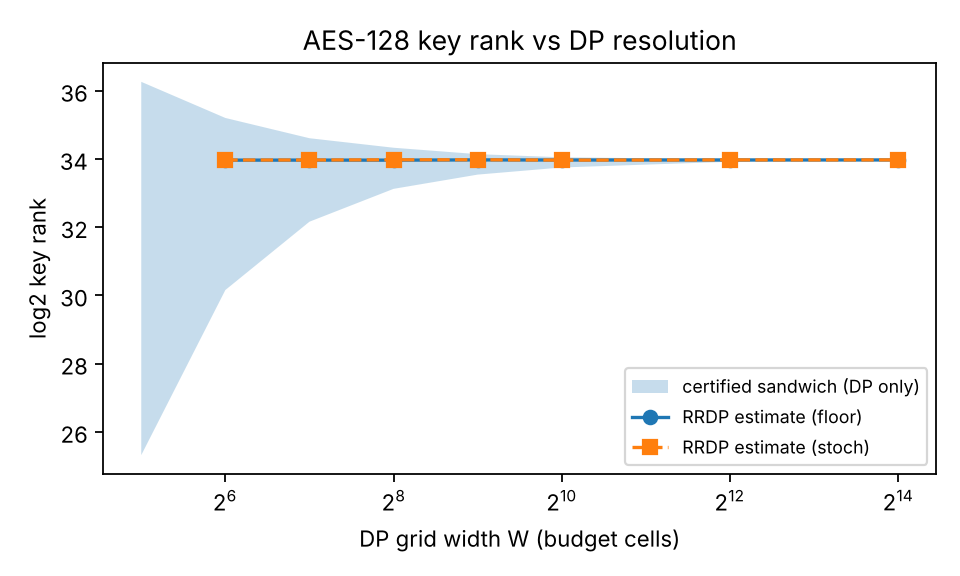
\includegraphics[width=.72\linewidth]{../results/aes_rank.png}
\caption{The deterministic sandwich narrows only as the DP is refined. The randomized correction
is accurate at every resolution where it runs.}\label{fig:aes}
\end{figure}

\paragraph{Floor vs.\ stochastic rounding.} We used synthetic exponential scores, $K=16$, $W=16m$, a partially
leaked key, and $2\cdot10^4$ samples per point.

\begin{table}[h]\centering\small
\resizebox{\linewidth}{!}{\begin{tabular}{@{}rccccc@{}}
\toprule
$m$ & mean floor bias $/D$ ($=m/2$) & stochastic slack $\tau/D$ & acceptance (floor) & acceptance (stoch.) & sample saving \\ \midrule
8 & 4.0 & 4.29 & 0.939 & 0.922 & $0.98\times$ \\
16 & 8.0 & 6.07 & 0.788 & 0.809 & $1.03\times$ \\
32 & 16.0 & 8.58 & 0.614 & 0.776 & $1.26\times$ \\
64 & 32.0 & 12.14 & 0.410 & 0.620 & $1.51\times$ \\
128 & 64.0 & 17.17 & 0.150 & 0.521 & $3.48\times$ \\ \bottomrule
\end{tabular}}
\caption{Stochastic rounding wins once $\sqrt{m\ln(1/\eta)/2}<m/2$, here at about $m\ge16$, as Lemma~\ref{lem:stoch} predicts.}\label{tab:scaling}
\end{table}

\subsection{Findings}
\begin{enumerate}[leftmargin=*]
\item \textbf{RQ1, rounding plus DP.} The DP on a rounded instance yields a certified sandwich whose width is
      governed by $m$ grid cells (Lemma~\ref{lem:sandwich}). It is reliable but biased, and coarse grids give loose bounds
      (10.9 bits at $W=32$).
\item \textbf{RQ2, randomized correction.} Sampling exactly from the rounded DP and rejecting removes the bias
      \emph{completely}: $\E[\hat R]=R$, with $(1\pm\eps)$ accuracy (Theorem~\ref{thm:floor}). A Dyer-type injection bound
      (Lemma~\ref{lem:dyer}) makes this an FPRAS for key rank, which is a \#P-hard problem (Corollary~\ref{cor:fpras}, Proposition~\ref{prop:hard}).
\item \textbf{RQ3, randomized rounding of inputs.} Unbiased shared-shift rounding cuts the error band from $\Theta(mD)$ to
      $O(D\sqrt{m\log(1/\eta)})$ at the cost of a one-sided bias of at most $\eta R$ (Theorem~\ref{thm:stoch}). It pays off for
      many subkeys (up to $3.5\times$ fewer samples at $m=128$) but not for $m\le16$.
\item \textbf{An honest caveat for AES-128.} With $m=16$ the DP is so cheap that a fine grid ($W=16384$) is the fastest
      option overall. Randomized rounding matters when the DP width is the bottleneck: many subkeys (bit-level or
      AES-256 / post-quantum key schedules), multi-constraint DPs, or tight memory such as on-device evaluation.
\end{enumerate}

\noindent In one line: \emph{rounding makes the DP small, the DP makes exact sampling possible, and
sampling makes the rounding error vanish in expectation.}

\section{Gaps and Future Directions}\label{sec:future}

\subsection{Gaps in this work}
\begin{enumerate}[leftmargin=*]
\item \textbf{Conservative sample size.} $n$ is set from the certified $p_{\mathrm{lo}}$, not from the true $p$. In
      Table~\ref{tab:aes} at $W=64$ we have $p_{\mathrm{lo}}=0.03$ while the realised $p=R/N(t^\star)\approx2^{33.97-35.20}\approx0.43$, so about $14\times$ too many samples were drawn.
\item \textbf{Weak certificate in stochastic mode.} Theorem~\ref{thm:stoch} still bounds $p'$ through the $m$-cell floor band.
      Its sampling advantage is therefore only realised with adaptive stopping (item~1 below).
\item \textbf{Worst-case constants.} Lemma~\ref{lem:dyer} gives $p\ge1/(m(K-1)+1)\approx1/4081$ for AES, which is far from the
      observed $0.4$--$0.99$. The FPRAS bound is correct but pessimistic.
\item \textbf{Independence assumption.} Additive scores assume independent subkey posteriors. Masked implementations,
      multivariate or joint templates, and key-schedule leakage couple the subkeys.
\item \textbf{Simulated leakage only.} The experiments use a Gaussian Hamming-weight model, not real traces or neural-network posteriors.
\end{enumerate}

\subsection{Future directions}
\begin{enumerate}[leftmargin=*]
\item \textbf{Adaptive sampling.} Replace the fixed $n$ by the Dagum--Karp--Luby--Ross stopping rule~\cite{dklr2000}: about
      $O(\eps^{-2}p^{-1}\log\delta^{-1})$ samples in expectation using the \emph{true} $p$. This closes gaps~1 and~2.
\item \textbf{Sharper rounding analysis.} Dyer refines the basic bound to $\tilde O(n^{2.5}+n^2\eps^{-2})$ and points to further gains
      from randomized rounding~\cite{dyer2003}. Feng and Jin reach \emph{subquadratic} time for \#Knapsack within Dyer's framework,
      working on a randomly rounded instance~\cite{feng2025}. Lifting these to the multiple-choice (key-rank) case is open.
\item \textbf{Deterministic FPTAS for key rank.} Combine Lemma~\ref{lem:dyer} with approximate-count DPs over read-once branching
      programs~\cite{gopalan2011,stefankovic2012} to remove randomness while keeping polynomial time.
\item \textbf{Coupled subkeys.} Run the DP over a tree decomposition of the dependency graph between subkeys (for example,
      second-order masking pairs). The cost becomes exponential only in the treewidth.
\item \textbf{Sampling as enumeration.} The exact sampler over $S'$ gives a \emph{randomized key search} with a provable
      success probability per guess. That suggests GPU-parallel, stateless enumeration in the spirit of~\cite{martin2015,poussier2016}.
\item \textbf{Deep-learning SCA.} Plug calibrated network posteriors (ASCAD~\cite{benadjila2020}) into \textsc{RRDP-Rank}. An open question is
      how model miscalibration compares with rounding error, and whether stochastic rounding acts as a regulariser.
\item \textbf{Equality constraints.} Counting $\{x: a\cdot x=t\}$ (subset-sum preimages, relevant to the density of
      Merkle--Hellman-type keys~\cite{merkle1978,lagarias1985}) defeats ratio-based estimation, because $|A|$ can be $0$. Finding rounding schemes with
      guarantees for this case is open.
\item \textbf{Leakage of the evaluator.} The DP and sampler are data-dependent. If run on-device, they should be
      constant-time, or the rank estimator itself becomes a side channel.
\end{enumerate}


\appendix
\section{Reproducibility}
All code is in \texttt{code/} (Python~3, NumPy, Matplotlib).
\begin{itemize}[nosep]
\item \texttt{python3 test\_rrdp.py}: checks the lemmas and theorems against brute force.
\item \texttt{python3 experiment\_aes.py}: AES-128 experiment (Table~\ref{tab:aes}, Fig.~\ref{fig:aes}).
\item \texttt{python3 experiment\_scaling\_m.py}: floor vs.\ stochastic rounding (Table~\ref{tab:scaling}).
\end{itemize}
Real scores are converted to exact \texttt{int64} fixed point (resolution $2^{-20}$ nats), so
all cost comparisons are exact. Counts are \texttt{float64}. All terms are non-negative, so the
relative error is at most about $mK\cdot2^{-53}$, and counts are exact below $2^{53}$.

\bibliographystyle{plain}
\bibliography{refs}
\end{document}
